\documentclass[a4paper,14pt]{article}
\usepackage{extsizes}
\usepackage[english, russian]{babel}
\usepackage[pdftex]{graphicx}
\usepackage[T2A, T1]{fontenc}
\usepackage[utf8]{inputenc}
\usepackage{caption}
\usepackage{amsthm}
\usepackage{amsmath}
\usepackage{amsfonts}
\usepackage{geometry}  % установка полей
\usepackage{cases}
\usepackage{cancel}
\usepackage[final]{pdfpages}
\geometry{top=3.5cm,bottom=2cm,left=2cm,right=2cm}
%\usepackage{graphicx}
\graphicspath{}
\DeclareGraphicsExtensions{.pdf,.png,.jpg,}
%\renewcommand{\figurename}{Рис}
\renewcommand{\figurename}{Рис.}
\renewcommand{\d}{\displaystyle}
%\renewcommand{\rmdefault}{ftm}
\newtheorem*{note}{Замечание} \theoremstyle{remark}
\newtheorem*{theorems}{Теорема}
\newtheorem*{conjecture}{Гипотеза}
\begin{document}
%\documentclass[a4paper,14pt]{article}
\usepackage{extsizes}
\usepackage[english, russian]{babel}
\usepackage[pdftex]{graphicx}
\usepackage[T2A, T1]{fontenc}
\usepackage[utf8]{inputenc}
\usepackage{caption}
\usepackage{amsthm}
\usepackage{amsmath}
\usepackage{amsfonts}
\usepackage{geometry}  % установка полей
\usepackage{cases}
\usepackage{cancel}
\usepackage[final]{pdfpages}
\geometry{top=1cm,bottom=1cm,left=1cm,right=1cm}
%\usepackage{graphicx}
\graphicspath{}
\DeclareGraphicsExtensions{.pdf,.png,.jpg,}
%\renewcommand{\figurename}{Рис}
\renewcommand{\figurename}{Рис.}
\renewcommand{\d}{\displaystyle}
%\renewcommand{\rmdefault}{ftm}
\newtheorem*{note}{Замечание} \theoremstyle{remark}
\newtheorem*{theorems}{Теорема}
\newtheorem*{conjecture}{Гипотеза}
\begin{document}
\begin{titlepage}
\begin{center}
ФЕДЕРАЛЬНОЕ ГОСУДАРСТВЕННОЕ БЮДЖЕТНОЕ ОБРАЗОВАТЕЛЬНОЕ \\*
УЧРЕЖДЕНИЕ ВЫСШЕГО ОБРАЗОВАНИЯ \\*
<<МОСКОВСКИЙ ГОСУДАРСТВЕННЫЙ УНИВЕРСИТЕТ \\*
имени М.В.ЛОМОНОСОВА>> \\*
\end{center}

\begin{center}
МЕХАНИКО-МАТЕМАТИЧЕСКИЙ ФАКУЛЬТЕТ \\*
\end{center}

\begin{center}
КАФЕДРА ГИДРОМЕХАНИКИ \\*
\end{center}

\begin{center}
\vspace{2cm}
ВЫПУСКНАЯ КВАЛИФИКАЦИОННАЯ РАБОТА \\*
(ДИПЛОМНАЯ РАБОТА) \\*
специалиста \\*
\end{center}

\begin{center}
\Large \textbf{Осаждение частиц при одномерных течениях суспензии в пористых средах}
\end{center}

\begin{center}
\Large \textbf{Particle deposition in one-dimensional flows of suspension through porous media}
\end{center}

\vspace{1cm}

\begin{flushright}
\begin{minipage}{10cm}
Выполнил студент \\*
624 группы \\*
А.П.Волчанский \\*
\vspace{1cm} \\*
\underline{\hspace{2in}} \\*
подпись студента\\
\end{minipage}
\end{flushright}

\begin{flushright}
\begin{minipage}{10cm}
Научный руководитель: \\*
доцент, кандидат ф.-м. наук \\*
Н.Е.Леонтьев \\*
\vspace{1cm} \\*
\underline{\hspace{2in}} \\*
подпись научного руководителя \\*
\end{minipage}
\end{flushright}

\vspace{1.5cm}

\begin{center}
Москва \\*
\vspace{0.5cm}
2018
\end{center}

\end{titlepage}
\end{document}
\begin{titlepage}
%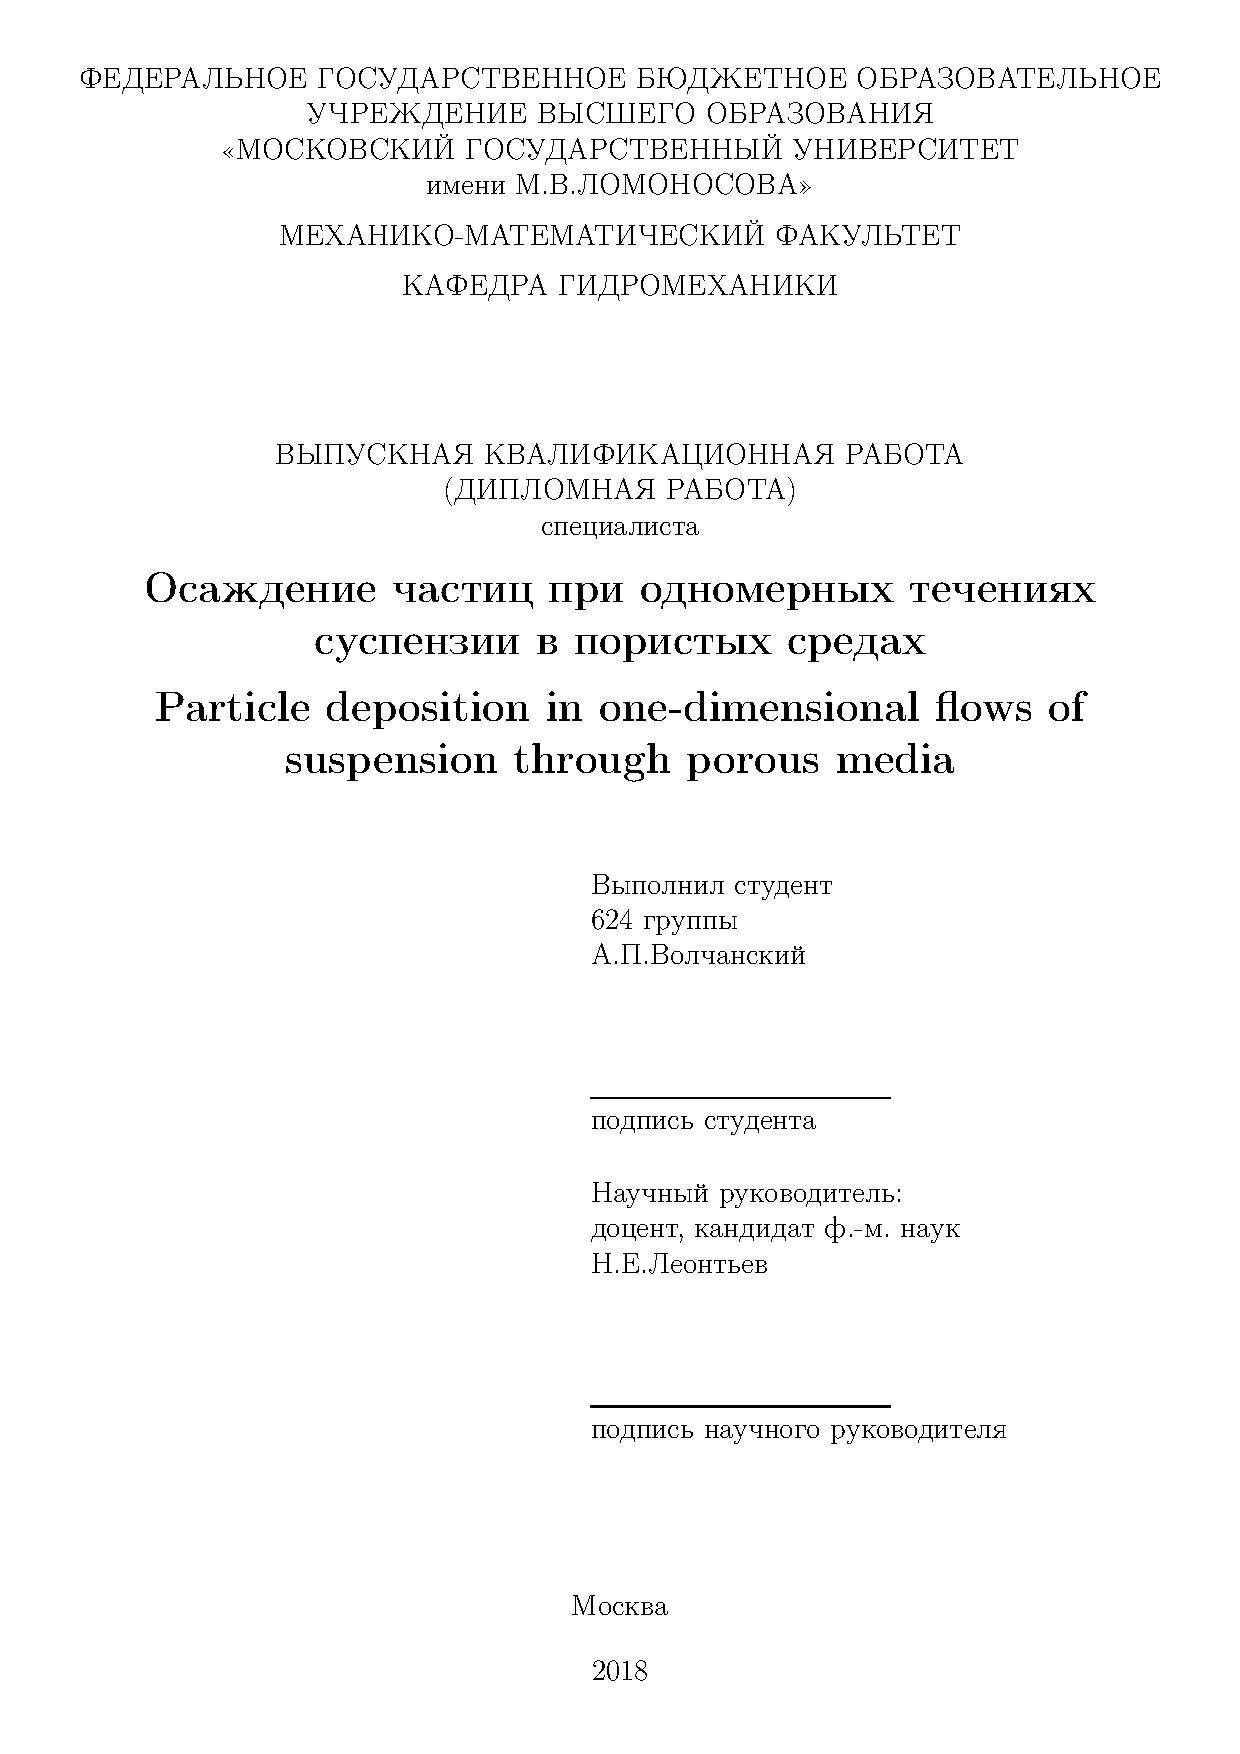
\includepdf[pages=-,pagecommand={},width=\textwidth]{titlepage_2.pdf}
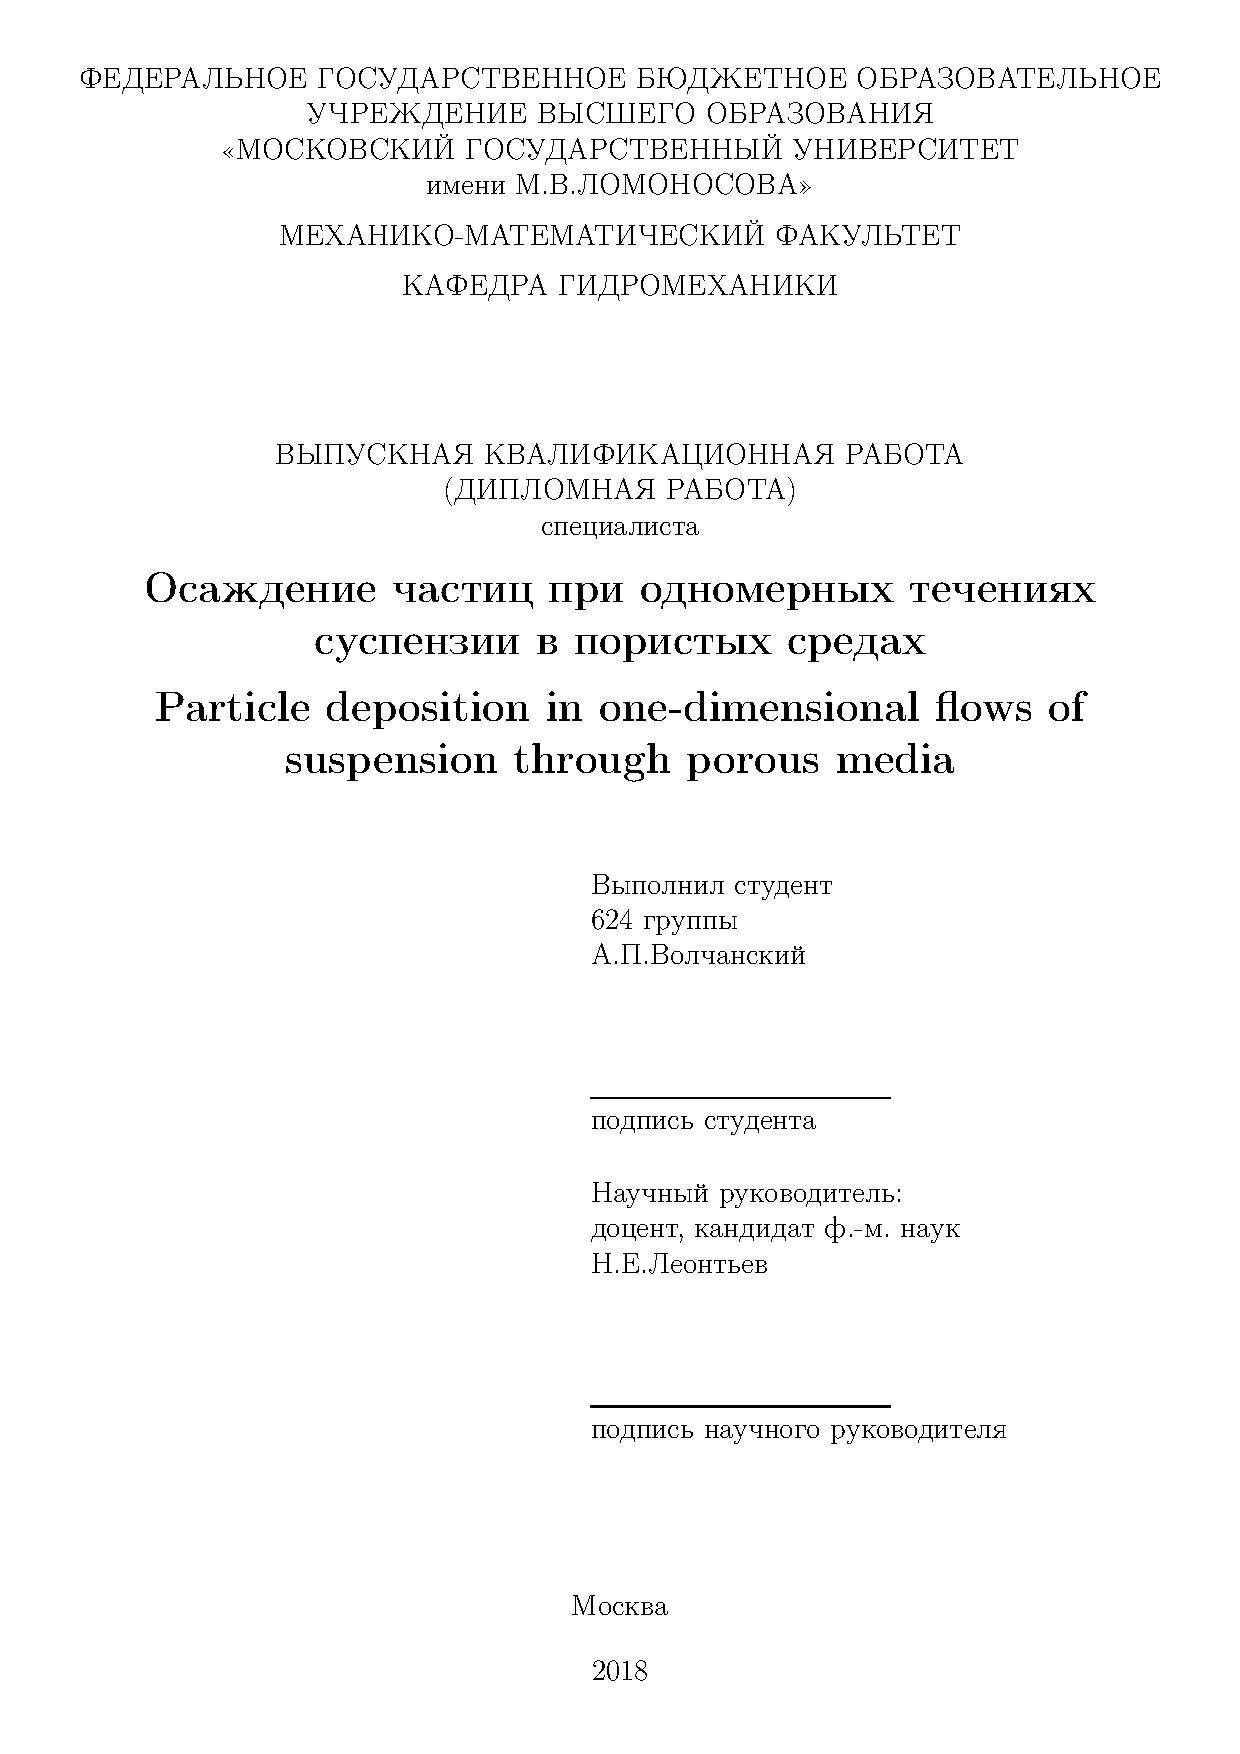
\includepdf[pages=-]{titlepage_2.pdf}
\end{titlepage}
\setcounter{page}{2}
\tableofcontents
\pagebreak
\section{Введение}

\par Одной из важных современных отраслей механики сплошной среды является теория фильтрации. Прикладное значение знаний, полученных во время изучения этой дисциплины, обусловлено большим значением энергетических и природных ресурсов, необходимых для жизни современного человечества. Такие отрасли, как нефтедобыча и очистка воды от примесей, являются сегодня одними из лидирующих в мире.
\par В большинстве природных процессов фильтрация жидкости сквозь пористую среду происходит при наличии в жидкости мелких в масштабах течения частиц. Примерами таких течений могут быть течение загрязнённой воды сквозь очищающий слой фильтра, закачка пропанта в трещину после её создания методом гидроразрыва пласта.
\par Характерными особенностями таких задач являются движение мелких частиц в относительно высоких концентрациях, которое происходит со скоростями, равными скорости несущего флюида, и загрязнение фильтрующего пласта, которое сопровождается изменением пористости и других параметров.
\par Целью работы является изучение таких важных процессов для описания такой задачи, как отложение частиц на поверхности пористого скелета и их диффузия в процессе движения. Также исследуются различные модели течения жидкости и оседания частиц на поверхности порового пространства.
\par  В данной работе была рассмотрена одномерная модель загрязнения пласта, где загрязнение моделируется кинетическим уравнением, отложение частиц зависит от скорости жидкости, пористости и концентрации частиц, а также были получены решения для функций пористости и концентрации частиц.
\section{Обзор литературы}
\subsection{Фильтрация с осаждением}
\par В природе процессы фильтрации \cite{barenblatt} и \cite{basniev} чаще всего протекают при наличии в текущем флюиде примесей, размеры которых много меньше, чем размеры пор породы. Участие этих примесей в засорении может сказываться как на течении жидкости как таковой, влияя на её эффективные механические параметры, так и на объёмной доле пор, что также меняет картину течения. 
\par В статьях \cite{osiptsov_1} и \cite{osiptsov_2} рассмотрено влияние сопротивления жидкости и силы Архимеда на распределение частиц в ламинарном потоке несущей жидкости в течении внутри трещены гидроразрыва в приближении тонкого слоя. Распределение частиц полагается неоднородным, рассматривается двухфазная модель течения. В ходе работы проводится сравнение численной модели с упрощённой аналитической и с экспериментаьными данными.
\par В статье \cite{kuzmina} рассматриваются различные долгосрочные эффекты влияния оседания примесей на пористый скелет, а также предлагается метод анализа подобных задач на больших временах с использованием рядов. В качестве результата получается асимптотическое решение задачи вблизи фронта концентрации.
\par В статье \cite{civan} рассматриваются различные виды зависимости скорости изменения пористого скелета из-за  осаждения частиц на его поверхности и выноса их оттуда потоком флюида. Также в статье предлагается обобщение данных моделей при помощи эмпирических зависимостей. Уравнения основываются на уравнениях сплошной среды и статистических закономерностях, обобщающих эмпирические законы.
\subsection{Фильтрация с диффузией}
\par В статье \cite{brinkman} исследуется течение в высокопористых средах и обосновывается закон движения в подобном типе задач. Производится сравнение с экспериментальными данными и более простыми зависимостями.
\par В статье \cite{leighton} рассматривается влияние диффузии сферических частиц на эффективную вязкость суспензии как целого. Выводится аналитическая модель и сравнивается с экспериментальными данными.
\par В статье \cite{phillips} приводится описание исследования различных эффектов, связанных с диффузией частиц в потоке высококонцентрированной смеси, на различные характеристики течения. Рассматриваются две различные постановки задачи: течение Куэтта между двумя соосными вращающимися цилиндрами и течение в трубе под действием перепада давления. В этой работе выделяется три основных компоненты, описывающие диффузионный поток: хаотическое движение частиц, соударение между частицами и диффузия из более вязких слоёв в менее вязкие. Полученные зависимости сравниваются с экспериментальными данными.

\section{Основные уравнения}

\subsection{Определения теории фильтрации}

\par Основное явление, изучаемое в этой работе --- осаждение частиц на поверхности пористой среды. В ходе этого процесса частицы могут прикрепляться к пористому скелету, что влияет на течение жидкости и объём пустот в среде.\\
\par Пусть $\alpha(x^{i},t)$ --- объёмная концентрация взвешенных частиц, $m(x^{i},t)$ --- пористость, то есть отношение объёма пор к объёму малого участка среды.\\
\begin{figure}[h!]
\center{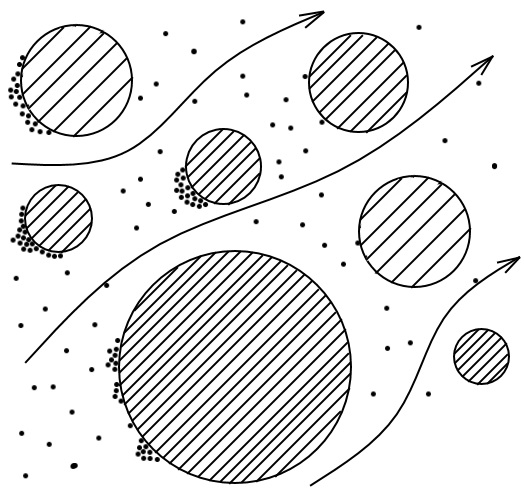
\includegraphics[width=7cm]{Particles_and_skeleton.jpg}}
\caption{Схема течения на уровне пор}
\label{fig:image1}
\end{figure}
\par Предполагается, что частицы имеют размер много меньше размера пор (во многих приложениях размер пор $d_{\text{ч}}\approx$ 1 мкм), перемещаются только благодаря потоку жидкости, перемешивание отсутствует. Это означает, что скорость частиц равна скорости жидкости. Также предполагается, что жидкость и частицы --- \textit{несжимаемые}, $\rho_{\text{ч}} = const, \; \rho_{\text{жидк}}\equiv\rho = const$.

\begin{figure}[h!]
\center{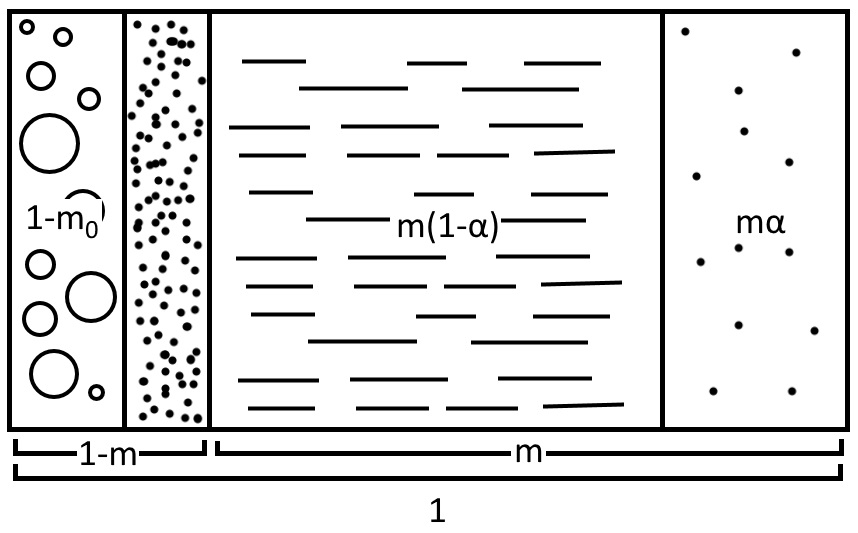
\includegraphics[width=10cm]{particles_quantity.jpg}}
\caption{Количество частиц в терминах $\alpha$ и $m$}
\label{fig:image2}
\end{figure}


\subsection{Законы сохранения массы}
\par Как и в других разделах механики сплошной среды, в теории фильтрации действуют стандартные законы сохранения. Их можно записать для каждой из фаз, для флюида и для частиц.
\par Запишем закон сохранения массы для жидкости:
$$\displaystyle \frac{d}{dt}\int\limits_{V}\rho m (1-\alpha)\,dV = - \int\limits_{\Sigma}\rho u_{n}(1-\alpha)\,d\sigma$$

\par Применяя стандартную технику перехода к дифференциальной форме, получим уравнение неразрывности для жидкой фракции:
$$
\begin{aligned}
\displaystyle 
\frac{\partial}{\partial t}(m(1-\alpha))+div((1-\alpha)\vec{u})=0
\end{aligned}
\eqno{(1)} 
$$
\par Также можно выписать соотношение на разрыве: 
$$[m(1-\alpha)]D-[(1-\alpha)u_{n}]=0$$
\par или в эквивалентной форме:
$$[m(\alpha-1)]D-[\alpha u_{n}]=0$$

\par Запишем аналогичный закон для частиц.

$$\displaystyle \frac{d}{dt}\int\limits_{V}{\rho_{\text{ч}}m\alpha+\rho_{\text{ч}}((1-m)-1-m_{0})}dV=-\int\limits_{\Sigma}\rho_{\text{ч}}\vec{u}\alpha d\sigma$$
\par Здесь $m_{0}=const$ --- первоначально пласт однородный. Перепишем полученные равенства в виде уравнения неразрывности:\\
$$(m\alpha)_{t}-m_{t}+div(\alpha \vec{u})=0$$
$$
\begin{aligned}
\displaystyle 
(m\alpha)_{t}+div(\alpha \vec{u})=m_{t}
\end{aligned}
\eqno{(2)} 
$$

\par Соотношение на разырыве:
$$[m\alpha-m]D-[\alpha u_{n}]=0$$

\par \textbf{Следствие:} Складывая (1)+(2) получаем уравнение неразрывности для \textbf{всей} суспензии.\\
$$m_{t}+div\;\vec{u}=m_{t}$$
$$div\;\vec{u}=0$$
\par Это уравнение можно использовать вместо (1) или (2) при решении системы уравнений.

\subsection{Закон Дарси}
\par В теории фильтрации используется экспериментальный закон Дарси, который связывает скорость и градиент давления. Этот закон можно получить как частное следствие закона Навье-Стокса при осреднении. Закон Дарси имеет вид:
$$
\begin{aligned}
\displaystyle 
-\vec{\nabla}P-\frac{\mu}{k}\vec{u}=0
\end{aligned}
\eqno{(3)} 
$$
\par В нашей постановке полагается, что массовых сил нет. В данной работе вязкость будет определяться в следующем виде:
$\mu=\mu(\alpha)=\mu_{0}(1+C\alpha)\approx\mu_{0},\;\;$
$k=k(m)$
\par В этой работе во многих задачах (3) отщепляется от системы.

\subsection{Кинетическое уравнение}

\par В исследуемой задаче функция, описывающая отложение частиц, считается известной, мы будем полагать, что данная зависимость имеет следующий вид:
$$
\begin{aligned}
\displaystyle 
m_{t}=-f(|\vec{u}|, m, \alpha)
\end{aligned}
\eqno{(4)} 
$$

\par С учётом кинетического уравнения мы можем выписать полную систему уравнений для поставленной задачи.

$$\displaystyle \begin {cases}
(m\alpha)'_{t}+(\alpha u)'_{x}=m'_{t}\\
u'_{x}=0\\
\displaystyle -P'_{x}-\frac{\mu}{k}u=0\\
m_{t}=-f(|\vec{u}|, m, \alpha)\\
\end {cases}$$

\subsection{Классификация системы уравнений}
\par В системе 6 уравнений и 6 неизвестных, $m, \alpha, P, \vec{u}$\\
\par Выписав систему уравнений для одномерных течений, можно получить матрицы с коэффициентами при производных переменных по $t$ (матрица $A_{ij}$) и по $x$ ($a_{ij}$). Если при этом у характеристического уравнения $|A_{ij}x-a_{ij}|=0$ все корни действительные, то система гиперболическая. Из этого следует, что уравнения в системе в характеристическом виде содержат производные по одному направлению (для каждого уравнения). Для нашей системы:\\
\bigskip
\\
$
\begin{cases}
\begin{aligned}
&(m\alpha)'_{t}+(\alpha u_{0})'_{x}=m'_{t}\\
&m_{t}=-f(|\vec{u}|, m, \alpha)
\end{aligned}
\end{cases}$
$\Leftrightarrow$
$
\begin{cases}
\begin{aligned}
&m\alpha'_{t}+\alpha m'_{t}+u_{0}\alpha'_{x}=m'_{t}\\
&m_{t}=-f(|\vec{u}|, m, \alpha)
\end{aligned}
\end{cases}$\\
\medskip
$\\
\begin{cases}
\begin{aligned}
&m\alpha'_{t}+(\alpha-1) m'_{t}+u_{0}\alpha'_{x}=0\\
&m_{t}=-f(|\vec{u}|, m, \alpha)
\end{aligned}
\end{cases}$
$\Leftrightarrow$
$
\begin{cases}
\begin{aligned}
&m\alpha'_{t}+u_{0}\alpha'_{x}=(\alpha-1)f(|\vec{u}|, m, \alpha)\\
&m_{t}=-f(|\vec{u}|, m, \alpha)
\end{aligned}
\end{cases}$\\
\bigskip
\\
\par Можно разделить производные (в каждом уравнении производные вдоль своего направления), значит система гиперболическая.
\section{Постановка задачи}
\subsection{Одномерное течение}
\par В этой работе рассматривается одномерное течение жидкости с частицами сквозь пористую среду. Выпишем систему уравнений для одномерного течения:
$$\displaystyle \begin {cases}
(m\alpha)'_{t}+(\alpha u)'_{x}=m'_{t}\\
u'_{x}=0\\
\displaystyle -P'_{x}-\frac{\mu}{k}u=0\\
m_{t}=-f(|\vec{u}|, m, \alpha)\\
\end {cases}$$

\par Сделаем следующие предположения. Пусть скорость $u=u_{0}=const$. Получили следующую систему:\\
$$\begin {cases}
(m\alpha)_{t}+\alpha_{x}u_{0}=m_{t}\\
m_{t}=-f(|\vec{u}|, m, \alpha)
\end{cases}$$
\par Получившаяся в результате предположений система является квазилинейной и содержит две неизвестные.

\subsection{Граничные условия}
\par В задаче рассматриваются следующие граничные условия:
\par \textbf{На входе} в пласт положим заданной концентрацию частиц $\alpha|_{x=0}=\alpha_{0}(t)$ и, в частности, $\alpha_{0}=const$\\
\par В начальный момент времени $t=0$ считаем заданной пористость среды  $m=m_{0},\text{а концентрацию}\;\;\alpha=0$ --- внутри пористой среды первоначально \textbf{чистая} жидкость.\\
\par \textbf{На выходе} из пласта при $x=L$ условия не ставятся, что связано с поведением характеристик.\\
\pagebreak
\subsection{Начало закачки в пласт}
\par На иллюстрации схематически показана зависимость $m$ и $\alpha$ от координаты $x$ в различные моменты времени $t_{i}$:
\begin{figure}[h!]
\center{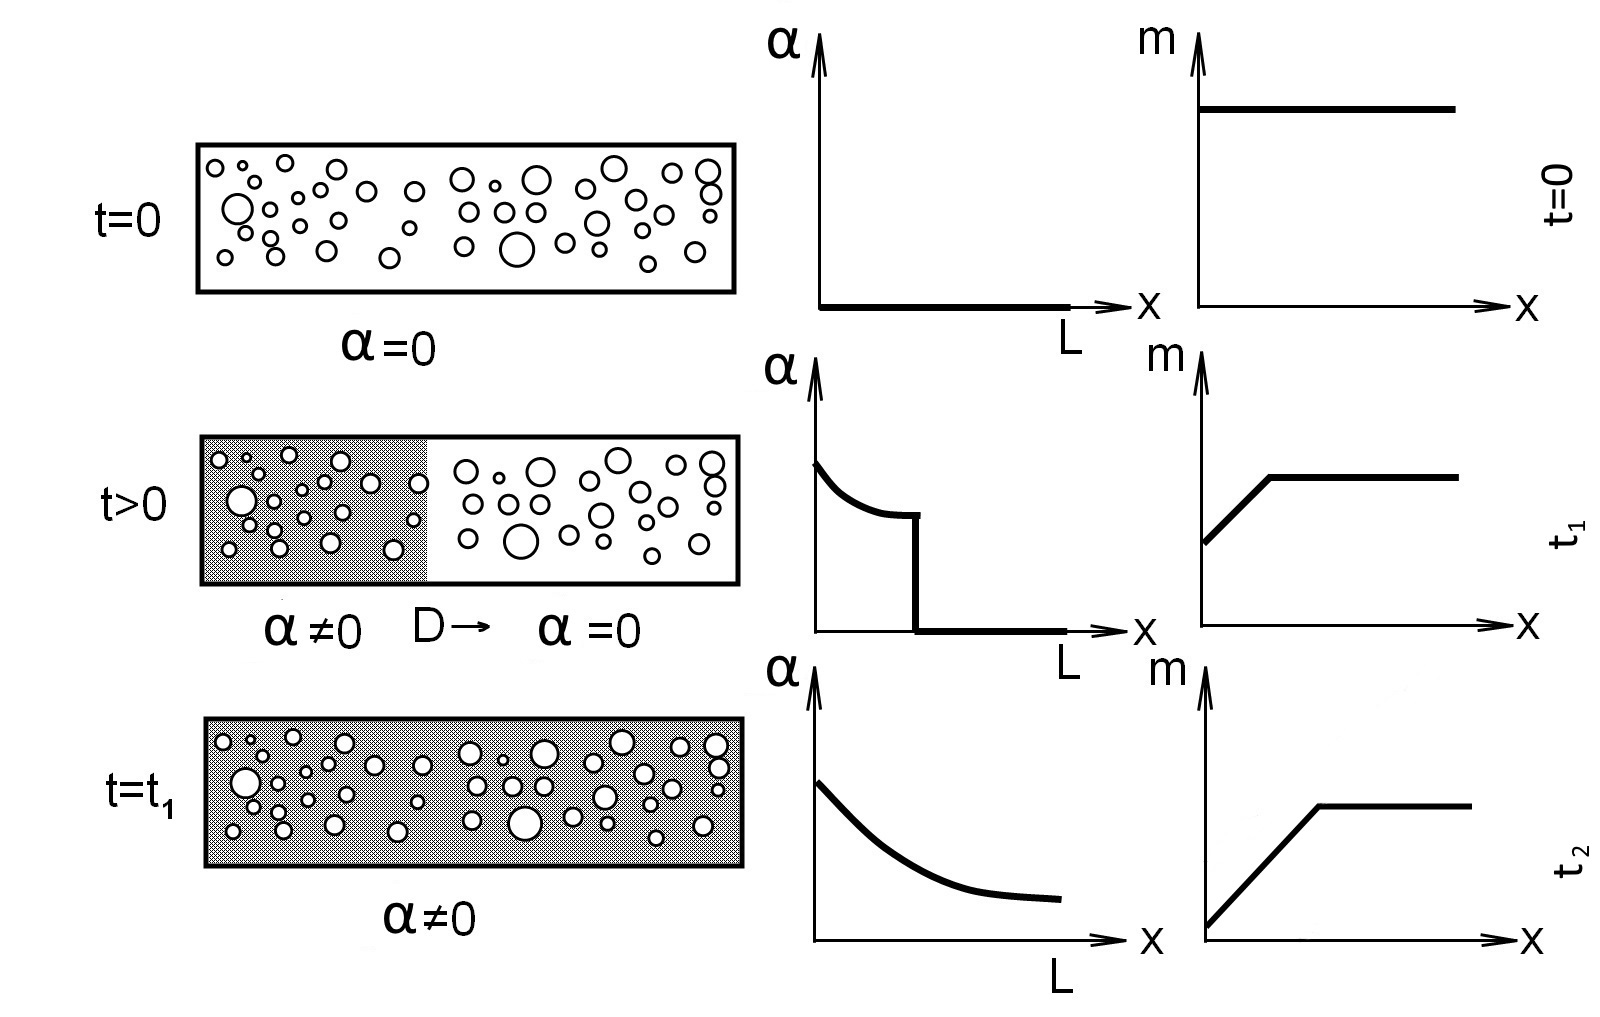
\includegraphics[width=15cm]{begining_of_loading.jpg}}
\caption{}
\label{fig:image1}
\end{figure}
\section{Решение упрощённой задачи с конкретным уравнением засорения}
\subsection{Дополнительные предположения}
\par Предположим, что $m\approx m_{0}$, то есть изменение пористости можно считать малым. Также можно предположить, что $\alpha\ll 1$ --- концентрация мала. Тогда от уравнения $$m_{t}\alpha + m\alpha+u_{0}\alpha_{x}=m_{t}$$ можно перейти к $$m_{0}\alpha_{t}+u_{0}\alpha_{x}=m_{t}$$ Добавим в систему частный случай кинетического уравнения засорения: $m_{t}=-\gamma \alpha |u_{0}|$, где множитель $\alpha |u_{0}|$ пропорционален объёму жидкости, протекающей через данную точку, а $\gamma=const$ --- экспериментальный коэффициент, который, например, в общем случае может зависеть от пористости. Далее мы проверим, что система имеет решение $\alpha=\alpha(x)$ за фронтом (не зависит от $t$, однако $m$ от времени зависит).\\
\par В итоге получаем уравнение $$\alpha'_{t}+\frac{u_{0}}{m_{0}}\alpha'_{x}=-\frac{\gamma\alpha |u_{0}|}{m_{0}}$$ 
\par Уравнению засорения соответствует характеристика $\d \frac{dx}{dt}=const$, а уравнению выше --- $\d\frac{dx}{dt}=\frac{u_{0}}{m_{0}}$. Поскольку разрыв идёт вдоль второй характеристики, то от разрыва уходит только одна характеристика --- условие эволюционности выполняется. Выпишем соотношение на разрыве: $[m(1-\alpha)]D-[(1-\alpha)u_{n}]=0,$ где $u_{n}=u_{0}$. Тогда: $m_{0}[1-\alpha]\frac{u_{0}}{m_{0}}-[1-\alpha]u_{0}=0$. Здесь мы пользуемся гипотезой $[m]=0$, но возможны и другие ситуации. \\
\par Можно поставить следующую задачу: при заданной $\alpha|_{x=0}=\alpha_{0}$ найти решение $\alpha(x)$ за скачком, а также $m=m(x,t)$. 
\subsection{Решение поставленной задачи}
\par Найдём решение уравнения вдоль характеристики $\d \frac{dx}{dt}=0$: $$\d \alpha_{t}+\frac{u_{0}}{m_{0}}\alpha_{x}=-\frac{\gamma\alpha|u_{0}|}{m_{0}}$$ 
\par Отсюда получаем $\d \frac{d\alpha}{dt}=-\frac{\gamma\alpha|u_{0}|}{m_{0}}$. $\d \int\frac{d\alpha}{\alpha}=-\int\frac{\gamma|u_{0}|}{m_{0}}dt$, откуда окончательно получаем $$\d ln\;\alpha=-\frac{\gamma|u_{0}|}{m_{0}}t+C$$\\
\par Перепишем полученное решение в виде $\d ln\frac{\alpha}{\alpha_{0}}=-\frac{\gamma|u_{0}|}{m_{0}}(t-t_{0})$. Так же, вспоминая, что мы искали решение вдоль характеристики, из $\d \frac{dx}{dt}=\frac{u_{0}}{m_{0}}$ можем получить $\d x=\frac{u_{0}}{m_{0}}(t-t_{0})$. Это показывает, что найденное решение можно представить в виде $\alpha=\alpha_{0}e^{-\gamma x}$, или 
\begin{equation*}
\d
\alpha=
\begin{cases}
\d
\alpha_{0}e^{-\gamma x},\;\;& x<\frac{u_{0}}{m_{0}}t\\
0,\;\;& x\geq \frac{u_{0}}{m_{0}}t\\
\end{cases}
\end{equation*}
 Представляя это решение в виде $\d \alpha=\alpha_{0}e^{-\gamma \frac{u_{0}}{m_{0}}(t-t_{0})}$, можно получить, что скорость разрыва $\d D=\frac{u_{0}}{m_{0}}$. Проверим выпонение условия баланса массы на скачке: $[m(1-\alpha)]D-[(1-\alpha)u_{n}]=0$, откуда $m_{0}[1-\alpha]D-[1-\alpha]u_{n}=0$. Так как $m_{0}D-u_{n}=0$, то отсюда следует $u=u_{0}=const$\\
\par Величина $\gamma$ имеет размерность $[\gamma]=\textbf{1/м}$. Её можно трактовать как типичную длину засорения, так как величина $\alpha/\alpha_{0}$ падает в $e$ раз на расстоянии $1/\gamma$ от начала координат.\\
\par Также у нас осталось уравнение $m_{t}=-\gamma u_{0}\alpha$. С его помощью найдём решение 
\begin{equation*}
\d
m=m|_{t=0}+\int\limits^{t}_{0}m_{t}dt=m_{0}-\int\limits^{t}_{0}\gamma u_{0}\alpha dt=
\begin{cases}
\d
m_{0}-\gamma u_{0}\alpha(x)(t-\frac{xm_{0}}{u_{0}}),\;\;& x<\frac{u_{0}}{m_{0}}t\\
m_{0},\;\;& x\geq \frac{u_{0}}{m_{0}}t\\
\end{cases}
\end{equation*}
\section{Решение задачи без упрощений}
\subsection{Полное уравнение.}
\par Теперь получим решение в случае, когда уравнение неразрывности не упрощается. Имеем систему 
\begin{equation*}
\begin{cases}
(m\alpha)_{t}+u_{0}\alpha_{x}&= m_{t}\\
m_{t}&= -\gamma u_{0}\alpha\\
\end{cases}
\end{equation*}
\par Подставляя второе в первое и раскрывая скобки, получим $$\d \alpha_{t}+\frac{u_{0}}{m}\alpha_{x}=(\alpha-1)\gamma\frac{u_{0}}{m}\alpha$$
\par Рассматривая характеристики $\d \frac{dx}{dt}=\frac{u_{0}}{m}$ и интегрируя соотношение, получаем $\d \int \frac{d\alpha}{\alpha^{2}-\alpha}=\int\gamma dx=\int\frac{d(\alpha-1)}{\alpha-1}-\int\frac{d\alpha}{\alpha}$. Интегрируя и потенцируя, получаем окончательно выражение для $\alpha$:
\begin{equation*}
\d
\alpha=
\begin{cases}
\d
\frac{1}{1-\frac{\alpha_{0}-1}{\alpha_{0}}e^{\gamma x}},\;\;& x<\frac{u_{0}}{m}t\\
0,\;\;& x\geq \frac{u_{0}}{m}t\\
\end{cases}
\end{equation*}

\par Теперь, зная решение для $\alpha$, можно выразить $m$: $ \d
m= m|_{t=0}+\int\limits^{t}_{0}m_{t}dt=m_{0}+\int\limits^{t}_{0}\gamma u_{0}\alpha=m_{0}+\int\limits^{t}_{\frac{xm_{0}}{u_{0}}}\gamma u_{0}\frac{1}{1-\frac{\alpha_{0}-1}{\alpha_{0}}e^{\gamma x}} dt=$
\begin{equation*}
=
\begin{cases}
\d
m_{0}-\gamma u_{0}\frac{1}{1-\frac{\alpha_{0}-1}{\alpha_{0}}e^{\gamma x}}(t-\frac{xm_{0}}{u_{0}}),\;\;& x<\frac{u_{0}}{m_{0}}t\\
m_{0},\;\;& x\geq \frac{u_{0}}{m_{0}}t\\
\end{cases}
\end{equation*}

\par Можно заметить, что полученное решение при $\alpha_{0} \rightarrow 0$ переходит в полученное ранее выражение $$\d \alpha=\frac{1}{1-\frac{\alpha_{0}-1}{\alpha_{0}}e^{\gamma x}}\approx\frac{\alpha_{0}}{e^{\gamma x}}$$
\section{Решения в виде рядов}
%\subsection{Различия с решённой задачей}
\par Существует метод поиска точных решений путём разложения общего уравнения в ряд по концентрации осаждённых частиц. Если полагать, что скорость отложения частиц не просто пропорциональна  модулю скорости фильтрации, а есть некоторая функция пористости, то система переписывается следующим образом.

\par Обозначим концентрацию осаждённых частиц $s = (1-m_{0})-(1-m)$. Тогда нашу систему можно записать как:

\begin{equation*}
\begin{cases}
(a(s)\alpha+s)_{t}+(b(s)\alpha)_{x}&= 0\\
-(s)_{t}&=K(s)\alpha\\
\end{cases}
\end{equation*}

\par Сопоставим коэффициенты, зависящие от $s$ с обозначениями в решённых задачах. $a(s)$ --- $m$, $b(s)$ --- $u_{0}$, $K(s)$ --- $-\gamma u_{0}$. Полученные этим способом функции $s$ и $\alpha$ обобщают решение, полученное в рассмотренных предельных случаях. 

\par Полагая $K(s)=\varepsilon\Lambda(s)$, где $\varepsilon$ --- малый параметр и раскаладывая функции $a(s)$, $b(s)$ и $\Lambda(s)$ в ряды по $s$ в окрестности нуля. Это справедливо, так как всё ещё принята гипотеза о слабом засорении. Таким образом получим системы дифференциальных уравнений на коэффициенты рядов, решая которые можно получить решения необходимой точности в данном классе решений.
\par Решения ищутся в виде $s(x,t,\varepsilon)=\varepsilon s_{1}(x,t)+\varepsilon^{2} s_{2}(x,t)+...$
\par Выпишем эти системы для нескольких членов разложения:

\begin{equation*}
\varepsilon^{1}: 
\begin{cases}
(a_{0}\alpha_{1}+a_{1}\alpha_{0}s_{1})_{t}+(b_{0}\alpha_{1}+b_{1}\alpha_{0} s_{1})_{x}&= -\lambda_{0} \alpha_{0}\\
-(s_{1})_{t}&= - \lambda_{0} \alpha_{0}\\
\end{cases}
\end{equation*}

\begin{equation*}
\varepsilon^{2}: 
\begin{cases}
(a_{0}\alpha_{2}+a_{1}\alpha_{1}s_{1}+a_{2}\alpha_{0} s_{1}^{2}+a_{1}\alpha_{0}s_{2})_{t}+\\+(b_{0}\alpha_{2}+b_{1}\alpha_{1} s_{1}+b_{2}\alpha_{0}s_{1}^{2}+b_{1}\alpha_{0} s_{2})_{x}&= -(\lambda_{0} \alpha_{1}+\lambda_{1}\alpha_{0}s_{1})\\
-(s_{2})_{t}&= - (\lambda_{0} \alpha_{1}+\lambda_{1}\alpha_{0}s_{1})\\
\end{cases}
\end{equation*}

\par Решая последовательно эти системы методом характеристик можно получить искомое решение с необходимой наперёд заданной точностью.
\section{Расширенный класс решений}
\subsection{Система уравнений для обобщённого кинетического уравнения}
\par Ранее рассмотренное кинетическое уравнение имело довольно простой вид, а именно $m_{t} = -u_{0}\gamma \alpha$, теперь мы попробуем придать ему более общий вид. Как отмечалось ранее, функция, характеризующая изменение пористости со временем, зависит от пористости в текущий момент времени. Пусть теперь кинетическое уравнение имеет вид $m_{t} = -F(m)\alpha$, где $F(m)$ --- произвольная функция. Перепишем нашу систему уравнеий:
\begin{equation*}
\begin{cases}

(m\alpha)_{t}+ u_{0}\alpha_{x} &= m_{t}\\
m_{t} &= -F(m)\alpha\\

\end{cases}
\end{equation*}

\par В отличие от рассмотренных до этого задач, мы перейдём не к переменной $\alpha$, а к переменной $m$. Пусть $\d G(m) = -\frac{1}{F(m)}$. Тогда
$$\Big(m \big(G(m)m_{t} - 1\big)\Big)_{t} + u_{0}\big(G(m)m_{t}\big)_{x} = 0$$

\par Докажем, что $\big(G m_{t}\big)_{x} = \big(G m_{x}\big)_{t}$.\\
\par Действительно, $\d \big(G(m)m_{t}\big)_{x} = G_{m}m_{t}m_{x} + G m_{tx} = \big(G m_{x}\big)_{t}$, откуда следует, что в нашем уравнении можно поменять местами производные по времени и по координате, а именно, получим:
$$\Big(m \big(G(m)m_{t} - 1\big)\Big)_{t} + u_{0}\big(G(m)m_{x}\big)_{t} = 0$$
\par Данное уравнение можно проинтегрировать по времени. Получим:\\
$$m \big(G(m)m_{t} - 1\big) + u_{0}G(m)m_{x} = \Phi(x)$$
где $\Phi(x)$ --- произвольная функция.
\par Переписывая последнее уравнение, получим:
$$m_{t}+\frac{u_{0}}{m}m_{x}=\frac{m+\Phi(x)}{G(m)m}$$
\par Это уравнение гиперболическое. Решая его методом характеристик, можем получить выражение для пористости.\\
\begin{equation*}
\begin{cases}

\d \frac{dm}{dt} &= \d \frac{m+\Phi(x)}{G(m)m}\\
&\\
\d \frac{dx}{dt}&= \d \frac{u_{0}}{m}\\
&\\
m_{t} &= -F(m)\alpha\\

\end{cases}
\end{equation*}

\par Решением одной из упрощённых задач было выражение для $m$. Обозначим
$$\d \theta=\frac{t-\frac{xm_{0}}{u_{0}}}{1 - \frac{\alpha_{0}-1}{\alpha_{0}}e^{\gamma x}}$$
\par Тогда:\\
$$m=m_{0}-\gamma u_{0}\theta$$
\par Найдём такую функцию $\Phi(x)$, которая соответствует данному решению. $G(m)=-\frac{1}{\gamma u_{0}}$. Для удобства выпишем, чему равны производные этого решения:\\
$$m = m_{0} - \gamma u_{0}\theta(t-\frac{xm_{0}}{u_{0}})$$
$$m_{t} = -\gamma u_{0}\theta$$
$$m_{x} = \gamma u_{0}\theta\frac{m_{0}}{u_{0}}-\gamma u_{0}(t-\frac{xm_{0}}{u_{0}})\theta^{2}\frac{\alpha_{0}-1}{\alpha_{0}}e^{\gamma x}\gamma$$\\
\par Подставляя и приводя подобные, получим $\Phi(x)=-m_{0}$.
\par Теперь, имея всю необходимую информацию, можно попробовать решить расширенную систему уравнений, используя новые знания о функции $\Phi(x)$.

\begin{figure}[h!]
\center{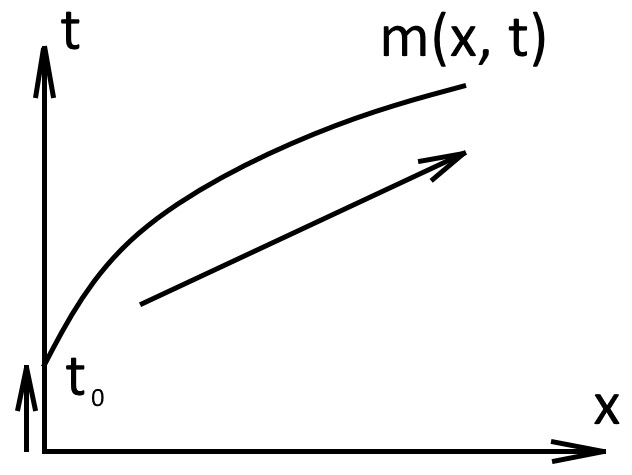
\includegraphics[width=7cm]{characteristics_solution_scheme.jpg}}
\caption{Схема решения методом характеристик.}
\label{fig:image1}
\end{figure}

\par В системе, которую мы уже писали раньше, заменим производную по времени производной по координате, что справедливо, поскольку мы находимся на характеристике.

\begin{equation*}
\begin{cases}

\d \frac{dm}{dx} &= \d \frac{m+\Phi(x)}{G(m)u_{0}}\\
&\\
\d \frac{dx}{dt}&= \d \frac{u_{0}}{m}\\
&\\
m_{t} &= -F(m)\alpha\\

\end{cases}
\end{equation*}

\par Запишем условия для нашей исходной задачи для функции $F(x)$ и граничные и начальные условия. Отсюда получается, что $\d G(x)=-\frac{1}{\gamma u_{0}}$, при $x=0$ концентрация частиц постоянна и равна $\alpha_{0}$, в начальный момент времени полагаем всюду пористость $m=m_{0} = const$.

\begin{equation*}
\begin{cases}

\d \frac{dm}{dx} = \d -\gamma (m+\Phi(x))\\
{}\\
\d \frac{dx}{dt}= \d \frac{u_{0}}{m}\\
{}\\
m_{t} = -\gamma u_{0}\alpha\\

\end{cases}
\end{equation*}

\par Получим решение в некотором параметрическом виде. Ход решения изображён на рис. 4. Сначала мы найдём, какая пористость будет на искомой характеристике при $x=0$ в момент времени $t = \hat{t}$. Решим первое уравнение в системе:

$$\frac{dm}{dx}=\gamma(m_{0}-m)$$
$$\frac{d(m_{0}-m)}{m_{0}-m}=-\gamma dx$$
$$ln(m_{0}-m)=-\gamma x + C$$
$$m_{0}-m = e^{c}e^{-\gamma x}$$
\par Теперь выразим $e^{c}$ через $m(\hat{t})$. На границе выполняется уравнение $m_{t}=-\alpha_{0}\gamma u_{0}$. Его решение имеет вид: 
$$m(x=0,t)=-\alpha_{0}\gamma u_{0}t+m_{0}$$
\par Значит, в момент времени $\hat{t}$ мы имеем пористость на входе в пласт, равную $m(x=0,\hat{t})=-\alpha_{0}\gamma u_{0}\hat{t}+m_{0}$. 
\par Используем его для нахождения произвольной постоянной:
$$m_{0}-m(x=0,\hat{t})= \alpha_{0}\gamma u_{0}\hat{t} = e^{c}$$
\par Получили выражение для $m(x,\hat{t})$:
$$m =m_{0} -\alpha_{0}\gamma u_{0}\hat{t}e^{-\gamma x}$$
\par Провести дальнейшую проверку планируется в последующей работе.

\par Вернёмся к этой задаче. Найдём $\Phi(x)$, если знаем, что решение имело вид $m=m_{0}-\gamma u_{0}\frac{t-\frac{xm_{0}}{u_{0}}}{1-\frac{\alpha_{0}-1}{\alpha_{0}}e^{\gamma x}}$.
\par На характиристике имели $\frac{dx}{dt}=\frac{u_{0}}{m}$, значит $x=\frac{u_{0}}{m}t+C$, тогда для кинетического уравнения $m_{t}=-\gamma u_{0}\alpha$ имеем:
$$m=m_{0}-\gamma u_{0}\frac{C}{1-\frac{\alpha_{0}-1}{\alpha_{0}}e^{\gamma x}}$$
$$\frac{dm}{dx}=-\gamma(m+\Phi(x))$$
\par Выпишем $\frac{dm}{dx}$:
$$\frac{dm}{dx}=-\gamma u_{0}C\frac{\alpha_{0}-1}{\alpha_{0}}\frac{e^{\gamma x}}{(1-\frac{\alpha_{0}-1}{\alpha_{0}}e^{\gamma x})^{2}}$$
\par Подставляем всё в уравнение и получаем выражение для $\Phi(x)$:
$$\Phi(x)=\gamma u_{0}\frac{C}{(1-\frac{\alpha_{0}-1}{\alpha_{0}}e^{gamma x})^{2}}-m_{0}$$
\par Проверка выполняется путём непосредственной подстановки полученной $\Phi(x)$ в исходное уравнение.
\par Параметр $C$ указывает на конкретную кривую, на которой искалось решение.
\section{Диффузия частиц в потоке в отсутствие оседания}
\subsection{Основные понятия}
\par Далее рассмотрим другой эффект: диффузию частиц. Как показано в \cite{phillips}, это может происходить по нескольким причинам.
\par Пусть $N_{b}$ --- поток частиц, связанный с броуновским движением, который пропорционален градиенту концентрации.
\par $N_{\mu}$ --- поток частиц, связанный с разницей в вязкости в различных слоях жидкости.
\par $N_{c}$ --- поток частиц, связанный со столкновением с другими объектами. В некоторых задачах рассматривается столкновение с частицами, мы же будем рассматривать столкновение с пористым скелетом.
\par Вообще говоря, механизмы диффузии крайне разнообразны. Их модели частично опираются на выводы из элементарной теории, частично  получаются эмпирически. В данной работе используется эмпирический подход, то есть строится не противоречащая наблюдаемым в повседневной жизни явлениям модель, которая далее будет применяться для получения простых аналитических результатов.
\par Далее будут рассмотрены задачи в средах, похожих на вату или сетку, в которых пористость велика. Такое приближение рассматривается ввиду того, что диффузия в низкопористых средах является моделью, полученной в результате осреднения более сложных процессов, механизм которых сильно отличается от диффузии в течении жидкости. Будем считать, что геометрия такова, что не может препятствовать миграции частиц в каком-либо направлении (среда изотропна).
\pagebreak
\section{Основные формулы и уравнения фильтрации с диффузией}
\subsection{Уравнение движения Бринкмана}
\par Ввиду того, что в рассмотрение вводятся среды, в которых пористость полагается большой, следует рассмотреть уравнение движение из \cite{brinkman}, которое будем называть законом фильтрации (или уравнением) Бринкмана: $$0 = - \vec{\nabla}p-\frac{\mu}{k}\vec{u}+\mu_{1}\Delta\vec{u}$$
\par Основная причина рассмотрения другого уравнения движения заключается в том, что закон Дарси рассматривает только действие пористого скелета на жидкий объём $(\sim \mu v/k)$, но не учитывает трение между слоями жидкости. По этой причине в уравнении движения оставляется член, связанный с вязким трением, а коэффициент $\mu_{1}$ определяется в \cite{brinkman} по следующей формуле: $$\mu_{1}=\mu(1+2{,}5 (1-m))$$.
\subsection{Компоненты общего потока диффузии}
\par Как уже говорилось выше, в этой работе рассматривается модель диффузии, которая может быть условно разделена на три составляющие:
\par 1) Броуновское движение частиц, связанное с множеством факторов, в том числое с хаотичностью устройства вутренней геометрии среды, которая была до получения осреднённых величин в теории фильтриции. $$\vec{N}_{b} = -D\vec{\nabla} \alpha$$
\par 2) Диффузия, связанная со столкновением частиц с пористым скелетом. Получена из следующего соображения: этот член диффузии линейно зависит от вариации числа столкновений частиц со скелетом, поторая в свою очередь пропорцианальна градиенту скорости частиц. Таким образом можем записать, приняв за $d$ характерный размер частиц пористого скелета или волокон:
$$\vec{N}_{c} = -Kd\vec{\nabla}(|u|\alpha)$$
\par 3) Диффузия, связанная с переменной вязкостью (!!!!!!!!!!!!!!!!!!!!!!!!!!!!!!!!!!!!)


\section{Задача о течении в высокопористой среде}
\par Рассмотрим подробнее задачу о течении в высокопористой среде, в которой используется уравнение Бринкмана.
\par Рассмотрим течение вязкой несжимаемой жидкости сквозь высокопористую среду. Пусть частицы могут осаждаться на стенки пористой среды. Тогда получим следующую систему уравнений:
\begin{equation*}
\begin{cases}
div\;\vec{u}= 0\\
-\vec{\nabla}p-\frac{\mu}{k}\vec{u}+\mu_{1}\Delta\vec{u}=0\\
(m\alpha)_{t}+div(\alpha\vec{u})=m_{t}+\cancelto{0}{D\Delta\alpha}\\
m_{t}=-\gamma \alpha |\vec{u}|\\
\end{cases}
\end{equation*}
\par В этой задаче полагаем, что засорение скелета мало, все коэффициенты --- постоянные.
\par Здесь мы рассмотрим следующую ситуацию: пусть скорость направлена по оси $x$, то есть
$$\vec{u}=u_{0}(y)\vec{e}_{x}$$
\par В этом приближении можем записать уравнение 
$$m_{0}\alpha'_{t}+u_{0}\alpha'_{x}=m_{t}+D(\cancelto{\text{\begin{scriptsize}
учёт диффузии в длинном тонком канале
\end{scriptsize}}}{\alpha''_{xx}}+\alpha''_{yy})$$
\par При $D=0$ получаем известное уже нам решение $\alpha = \alpha_{0}exp(-\gamma x)$, которое не зависит от $y$. Также, мы можем исследовать уравнение границы загрязнения:
$$\frac{dx_{f}}{dt}=\frac{u_{0}(y)}{m_{0}}$$
$$x_{f}=\frac{u_{0}(y)}{m_{0}}t=x_{f}(y,t)$$
\par Из последнего соотношения виден замечательный факт: со временем поверхность всё больше "размазывается".
\par Проверим условия на скачке: 
\begin{equation*}
\begin{cases}
[m]=0\\
[m(\alpha-1)]D-[\alpha u_{n}]=0\\
[u_{n}]=0\\
\end{cases}
\end{equation*}
\par Найдём скорость распространения границы $f = x-\frac{u_{0}(y)}{m_{0}}t=0$:
$$D=-\frac{f_{t}}{|\vec{\nabla}f|}=\frac{-\frac{u_{0}(y)}{m_{0}}}{\sqrt{1+(\frac{u'_{0}(y)}{m_{0}}t)^{2}}}=\frac{u_{0}}{\sqrt{m_{0}^{2}+(u'_{0}(y)t)^{2}}}$$
\par Найдём выражение для вектора нормали к поверхности раздела с "чистой" фазой:
$$\vec{n}=\frac{(1,-\frac{u_{0}'(y)}{m_{0}}t)}{\sqrt{1+(\frac{u'_{0}(y)}{m_{0}}t)^{2}}}=\frac{(m_{0}, -u'_{0}(y)t)}{\sqrt{m_{0}^{2}+(u'_{0}(y)t)^{2}}}$$
\par Используя полученные соотношения, проверим второе условие на скачке:
$$m_{0}[\alpha]\frac{u_{0}}{\sqrt{m_{0}^{2}+(u'_{0}(y)t)^{2}}}-[\alpha]\frac{u_{0}(y)m_{0}}{\sqrt{m_{0}^{2}+(u'_{0}(y)t)^{2}}}=0$$
\par Отсюда видно, что условие баланса массы автоматически выполняется.
\par Теперь получим само решение для $u_{0}(y)$. Запишем систему уравнений в декартовой системе координат, обозначив $\vec{u}=(u_{x}, u_{y})$:
\begin{equation*}
\begin{cases}
\d \frac{\partial u_{x}}{\partial x}+\cancelto{0}{\frac{\partial u_{y}}{\partial y}}=0\\
\d -\frac{\partial p}{\partial x}-\frac{\mu}{k}u_{x}+\mu_{1}\cancelto{0}{\frac{\partial^{2} u_{x}}{\partial x^{2}}}+\mu_{1}\frac{\partial^{2} u_{x}}{\partial y^{2}}=0\\
\d -\frac{\partial p}{\partial y}-\frac{\mu}{k}\cancelto{0}{u_{y}}+\mu_{1}\cancelto{0}{\frac{\partial^{2} u_{y}}{\partial x^{2}}}+\mu_{1}\cancelto{0}{\frac{\partial^{2} u_{y}}{\partial y^{2}}}=0\\
\end{cases}
\end{equation*}
\par Отсюда видно, что:\\
\par 1) Скорость зависит только от $y$.\\
\par 2) Давление зависит только от $x$.\\
\par Во втором уравнении перенесём давление в одну часть, а скорости в другую, то есть:
$$\frac{\partial p}{\partial x}=-\frac{\mu}{k}u_{x}+\mu_{1}\frac{\partial^{2} u_{x}}{\partial y^{2}}$$
\par Тогда видно, что левая и правая часть зависят от разных переменных. Это значит, что обе они одновременно равны одной и той же постоянной, которую мы обозначим $A$. Отсюда получаем, что давление линейно зависит от $x$:
$$P=Ax+C$$
\par Выпишем уравнение для профиля скорости:
$$\frac{\partial^{2} u_{x}}{\partial y^{2}}-\frac{\mu}{k\mu_{1}}u_{x}-\frac{A}{\mu_{1}}=0$$
\par Решение этого уравнения выглядит следующим образом:
$$u_{x}(y)=-\frac{Ak}{\mu}+C_{1}exp\;(\sqrt{\frac{\mu}{\mu_{1}k}y})+C_{2}exp\;(-\sqrt{\frac{\mu}{\mu_{1}k}y})$$
\par Величины $C_{1}$ и $C_{2}$ находятся из граничных условий. В этой задаче их два:\\
\par 1) Условие симметрии на расстоянии $h$ (ищем выражение для течения в канале)
$$\frac{\partial u_{x}}{\partial y}|_{y=h}=0$$
\par 2) Условие Навье проскальзывания на границе $y=0$: 
$$\frac{\partial u_{x}}{\partial y}|_{y=0}=bu_{x}|_{y=0}$$
\par Отсюда находим $C_{1}$ и $C_{2}$. Обозначим $\alpha=\frac{\mu}{\mu_{1}k}$. Тогда:
$$C_{1}=\frac{Abk}{h(b-\alpha+e^{2h\alpha}(b+\alpha))}$$
$$C_{2}=\frac{Abk}{h(b+\alpha+e^{-2h\alpha}(b-\alpha))}$$
\par [Построить графики с характерными параметрами, (b~0.1h)]

\section{Заключение}
\par В ходе работы была выписана система уравнений фильтрации для задачи течения суспензии сквозь пористую среду с эффектом отложения. Было получено два аналитических решения для системы уравнений. Было проведено знакомство с методами поиска решений путём разложения в ряд, а также была выполнена проверка этого метода на аналитическом решении. Была решена задача об обобщении кинетического уравнения, были получены параметры, соответствующие аналитическому решению. Также было проведено ознакомление с методом характеристик и с его помощью получены аналитические решения.

\begin{thebibliography}{99}
\bibitem{kuzmina}
Кузьмина Л.И., Осипов Ю.В.,
Асимптотика задачи фильтрации суспензии в поритой среде,
Вестник МГСУ, 2015, №1, с. 54-62
\bibitem{osiptsov_1}
Боронин С.А., Осипцов А.А.,
Влияние миграции частиц на течение суспензии в трещине гидроразрыва,
Известия Российской академии наук, Механика жидкости и газа, 2014, №2, с. 80-94
\bibitem{osiptsov_2}
Боронин С.А., Осипцов А.А.,
Двухконтинуальная модель течения суспензии в трещине гидроразрыва,
Доклады Академии наук, 2010, том 431, №6, с. 758-761
\bibitem{civan}
Civan F.,
Modified Formulations of Particle Deposition and Removal Kinetics in Saturated Porous Media,
Transport in Porous Media, 2016, vol. 111, pp. 381-410
\bibitem{leighton}
Leighton D., Acrivos A.,
The shear-induced migration of particles in concentrated suspensions,
Journal of Fluid Mechanics, 1987, vol. 181, pp. 415-439
\bibitem{phillips}
Phillips R.J., Armstrong R.C., Brown R.A. et al.,
A constitutive equation for concentrated suspensions that accounts for shearinduced particle migration,
Physics of Fluids, 1992, vol.4, pp. 30-40
\bibitem{barenblatt}
Баренблатт Г.И., Ентов В.М., Рыжик В.М.,
Движение жидкостей и газов в природных пластах, М., 
Недра, 1984
\bibitem{basniev}
Басниев К.С., Кочина И.Н., Максимов В.М.,
Подземная гидромеханика, М., 
Недра, 1993
\bibitem{brinkman}
Brinkman H.C.,
A calculation of the viscous force exerted by a flowing fluid on a dense swarm of particles,
Applied Scientific Research, 1949, Vol. 1, pp. 27-34
\bibitem{jeltov}
Желтов Ю.П.,
Механика нефтегазового пласта,
М., Недра, 1975

\end{thebibliography}

\end{document}